\section{Results} \label{sec:results}
Once the trees had been rooted, a general linear model with the normal family was constructed with the with expected number of substitutions as the input, and sampling time as the response. For all experiments using patient data, this fit was only over the plasma data, and the PBMCs expected subs were used as input. From this, we collected the difference between the observed sampling date, and the predicted date. 

\begin{figure}[!ht] \label{fig:results1}
	\centering
	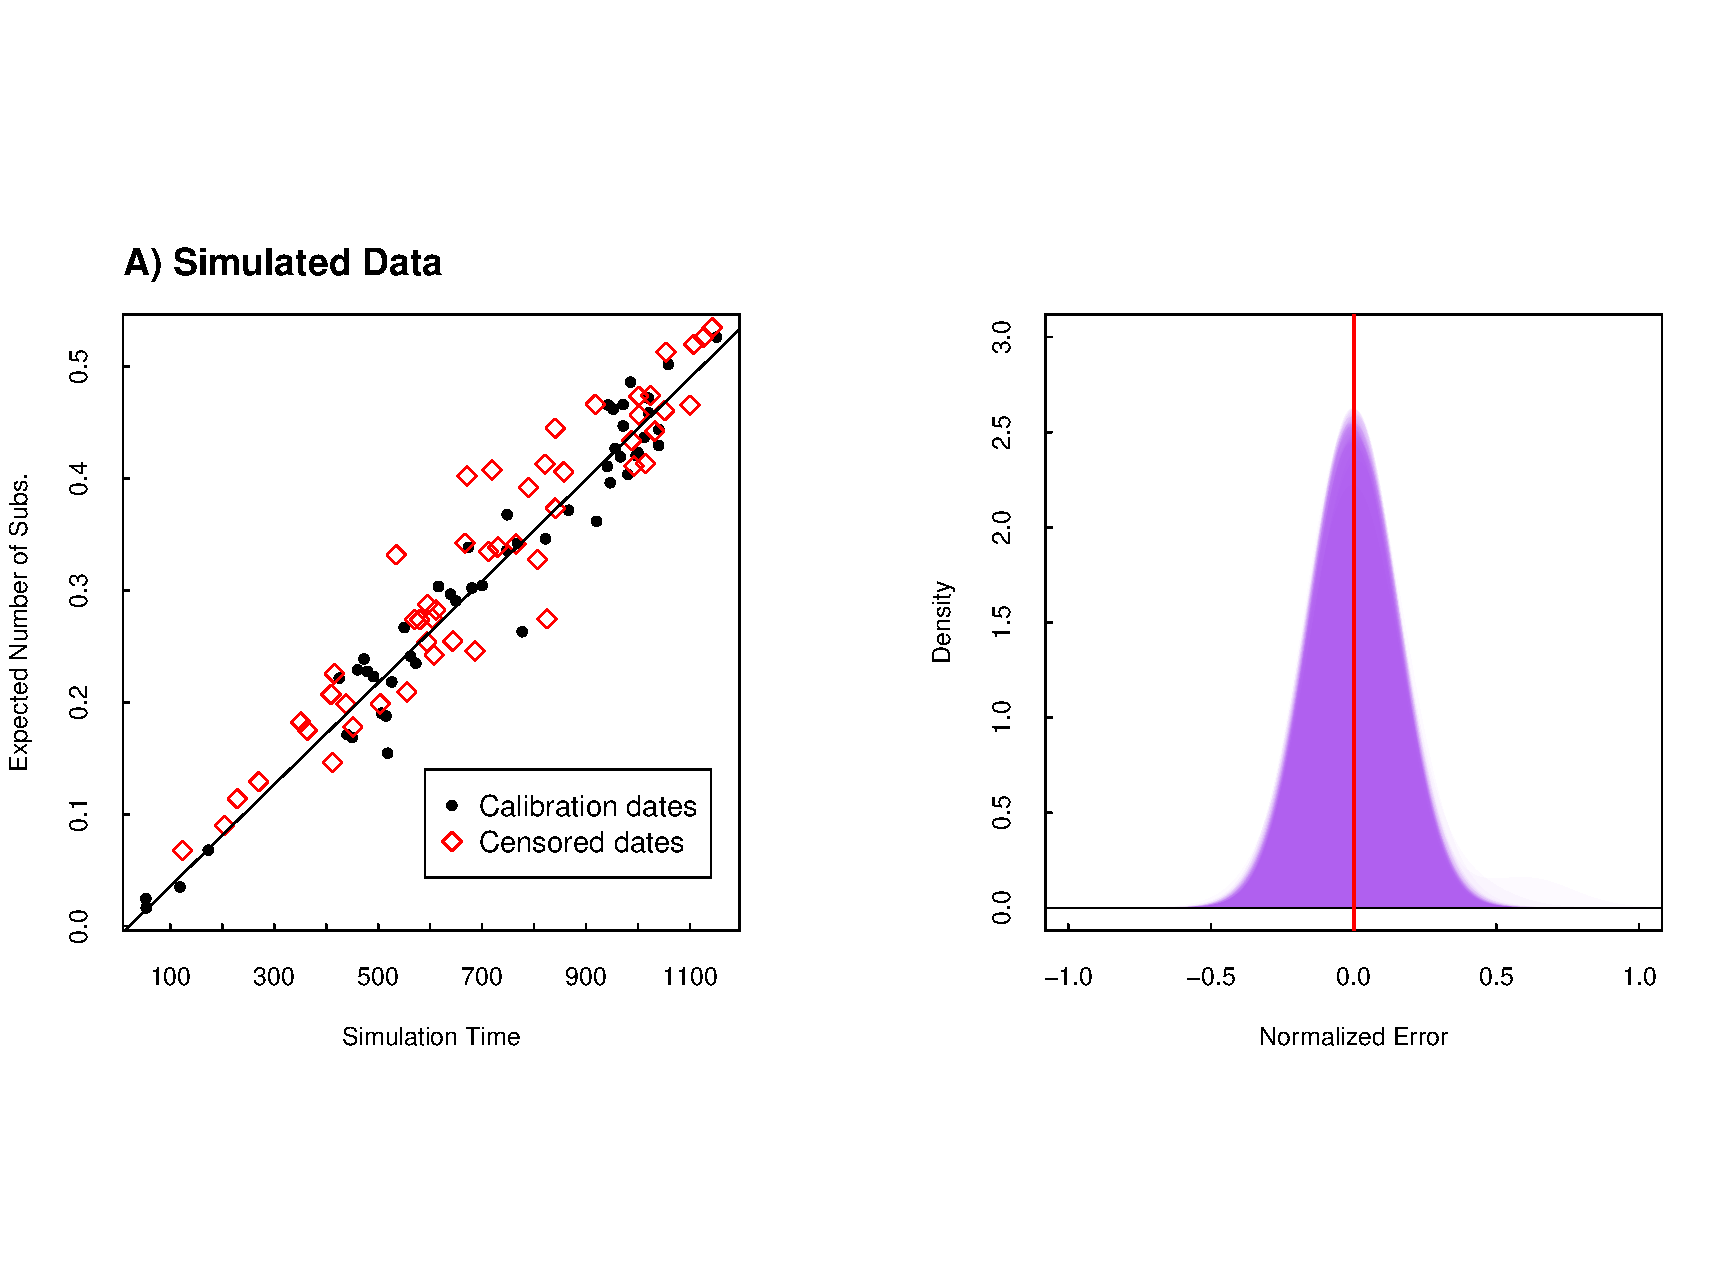
\includegraphics[trim=0cm 0cm 0cm 6cm, clip=true, scale=0.25]{figures/simulated.pdf} \\
	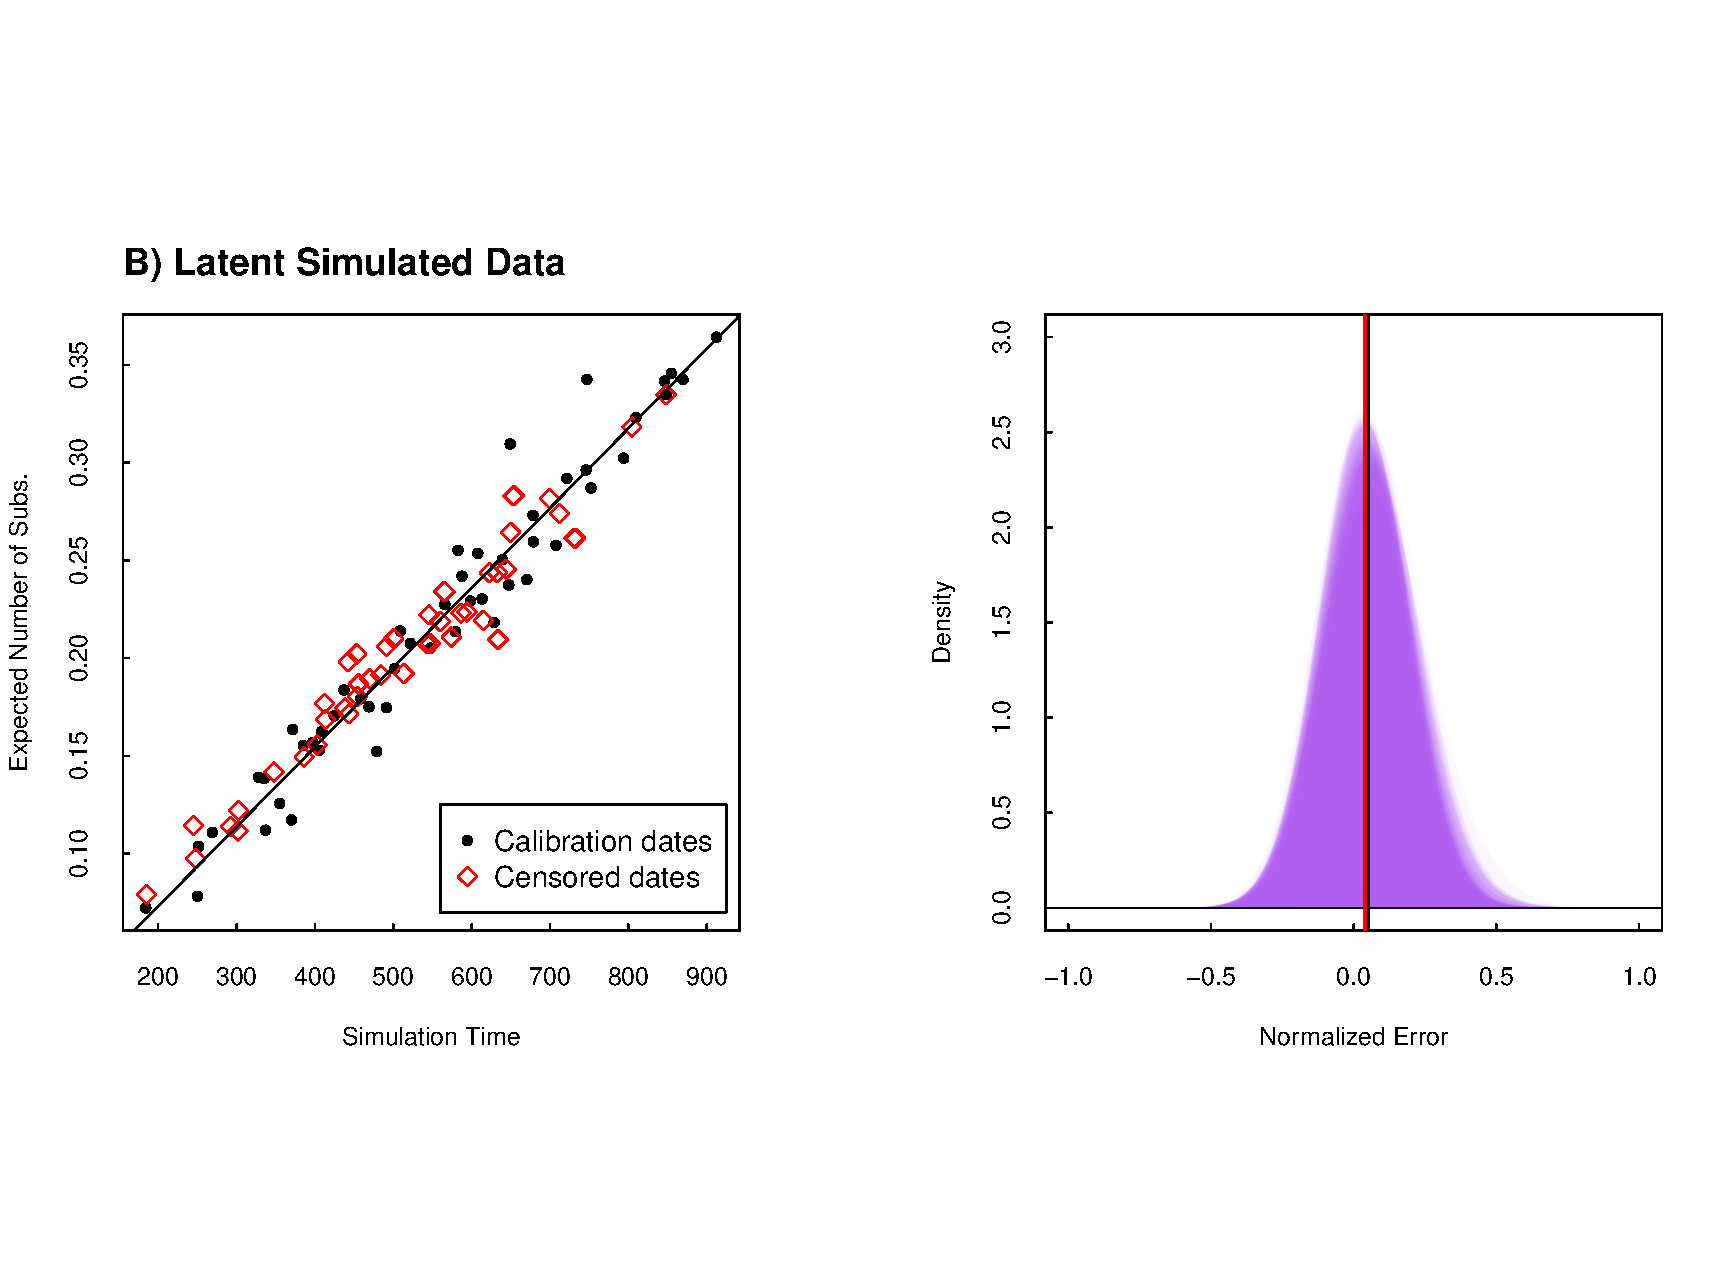
\includegraphics[trim=0cm 0cm 0cm 7cm, clip=true,scale=0.25]{figures/simulated_latent.pdf}\\
	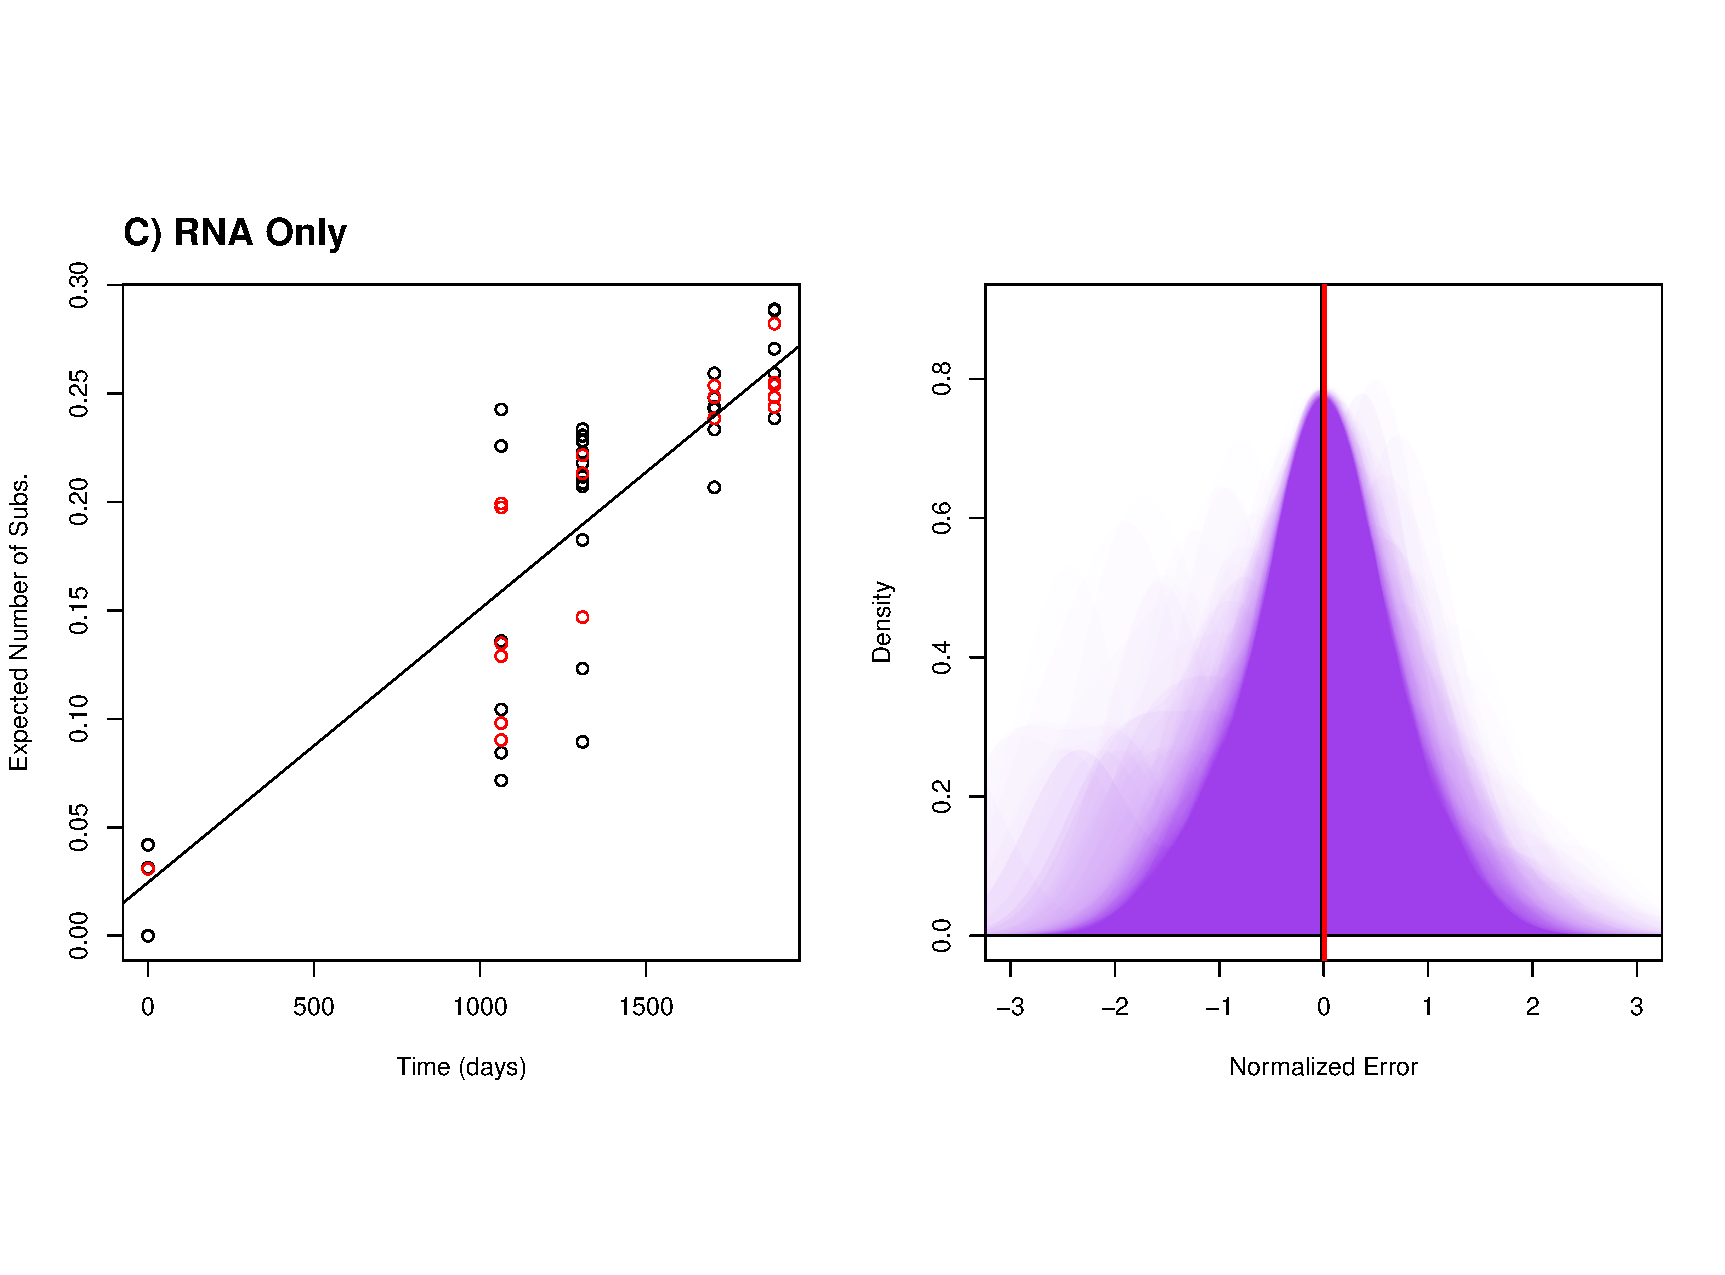
\includegraphics[trim=0cm 0cm 0cm 7cm, clip=true,scale=0.25]{figures/ancre.pdf}\\
	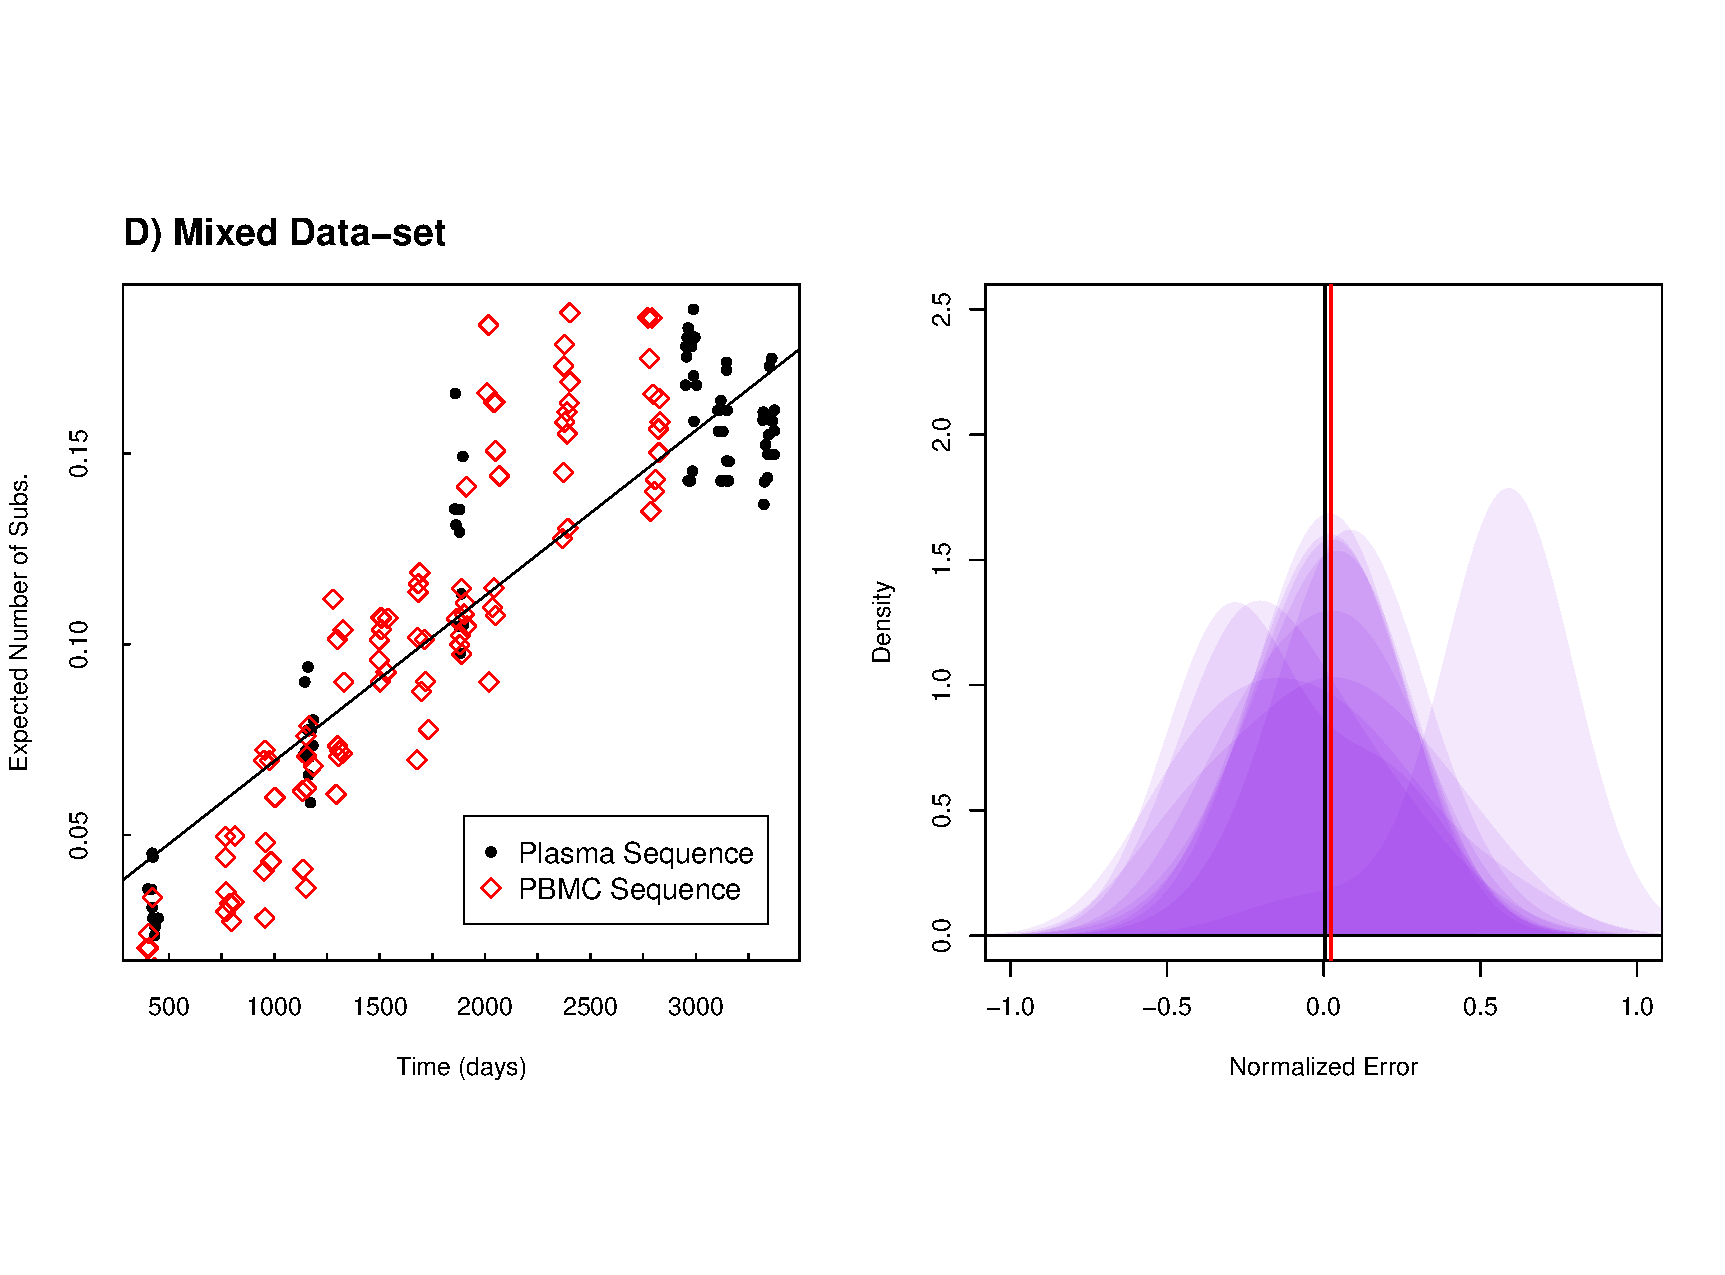
\includegraphics[trim=0cm 4cm 0cm 7cm, clip=true,scale=0.25]{figures/lanl.pdf}
	\caption[Examples]{Here's a set of examples}
\end{figure}


\subsection{Simulated Data} \label{sec:sim_results}
Summarize simulated data

\subsection{Simulated Latent Data} \label{sec:sim_lat_results}
Summarize


\subsection{RNA Only Data} \label{sec:rna_only}
summarize 

\subsection{Patient Reconstruction}
Summarize patient data

